% This is LLNCS.DEM the demonstration file of
% the LaTeX macro package from Springer-Verlag
% for Lecture Notes in Computer Science,
% version 2.4 for LaTeX2e as of 16. April 2010
%
\documentclass[a4paper,fontsize=11pt]{scrartcl}



% Anpassungen an DC Template
\usepackage[a4paper, left=2.9cm,right=2.87cm,bottom=3cm,top=3cm,headsep=1.27cm]{geometry}
\setlength{\parskip}{0.5em}
\renewcommand{\tablename}{TABLE} 
\renewcommand{\figurename}{FIG.} 
\usepackage{titlesec}
\titlespacing\section{0pt}{12pt plus 2pt minus 2pt}{6pt plus 1pt minus 1pt}
\titlespacing\subsection{0pt}{12pt plus 2pt minus 2pt}{3pt plus 1pt minus 1pt}
\addtokomafont{title}{\fontsize{14pt}{1em}\selectfont}
\setkomafont{section}{\fontsize{12pt}{0pt}\selectfont}
\addtokomafont{subsection}{\fontsize{11pt}{0pt}\selectfont}
% \addtokomafont{author}{\fontsize{12pt}{1em}\selectfont}
\usepackage{scrpage2}
\clearscrheadfoot
\pagestyle{scrheadings}
\renewcommand*{\titlepagestyle}{scrheadings}
\chead{\fontsize{9pt}{0pt}\selectfont Proc. Int'l Conf. on Dublin Core and Metadata Applications 2015}
\usepackage{apacite}


\date{}

\usepackage[utf8]{inputenc}

% URL handling
\usepackage{url}
\urlstyle{same}

% Todos
\usepackage[colorinlistoftodos]{todonotes}
\newcommand{\ke}[1]{\todo[size=\small, color=orange!40]{\textbf{Kai:} #1}}
\newcommand{\tb}[1]{\todo[size=\small, color=green!40]{\textbf{Thomas:} #1}}


% \usepackage{makeidx}  % allows for indexgeneration -- yes, but we don't need this

\usepackage{amsmath}

% monospace within text
\newcommand{\ms}[1]{\texttt{#1}}

% examples
\usepackage{fancyvrb}
\DefineVerbatimEnvironment{ex}{Verbatim}{numbers=left,numbersep=2mm,frame=single,fontsize=\scriptsize}

\usepackage{xspace}
% Einfache und doppelte Anfuehrungszeichen
\newcommand{\qs}{``} 
\newcommand{\qe}{''\xspace} 
\newcommand{\sqs}{`} 
\newcommand{\sqe}{'\xspace} 

% checkmark
\usepackage{tikz}
\def\checkmark{\tikz\fill[scale=0.4](0,.35) -- (.25,0) -- (1,.7) -- (.25,.15) -- cycle;} 

% Xs
\usepackage{pifont}

% Tabellenabstände kleiner
\setlength{\intextsep}{10pt} % Vertical space above & below [h] floats
\setlength{\textfloatsep}{10pt} % Vertical space below (above) [t] ([b]) floats
% \setlength{\abovecaptionskip}{0pt}
% \setlength{\belowcaptionskip}{0pt}

\usepackage{tabularx}
\newcommand{\hr}{\hline\noalign{\smallskip}} % für die horizontalen linien in tabellen

\newenvironment{DL}{
  %\scriptsize
  %\sffamily
  \vspace{0cm}
	\begin{center}
  \begin{tabular}{r l}

}{
  \end{tabular}
	\end{center}
}

% just makes the table prettier (see \toprule, \bottomrule, etc. commands below)
\usepackage{booktabs}

% Tabellenabstände kleiner
\setlength{\intextsep}{10pt} % Vertical space above & below [h] floats
\setlength{\textfloatsep}{10pt} % Vertical space below (above) [t] ([b]) floats
% \setlength{\abovecaptionskip}{0pt}
% \setlength{\belowcaptionskip}{0pt}

\usepackage{tabularx}

\usepackage{float}

\begin{document}

\title{\vspace{-1em}Guidance, please! Towards a framework for RDF-based constraint languages.}

\author{Thomas Bosch\\GESIS – Leibniz Institute \\for the Social Sciences, Germany\\thomas.bosch@gesis.org \and Kai Eckert\\Stuttgart Media University, Germany\\eckert@hdm-stuttgart.de}

\maketitle
\vspace{-3em}
\section*{Abstract}
In the context of the DCMI RDF Application Profile task group and the W3C Data Shapes Working Group solutions for the proper formulation of constraints and validation of RDF data on these constraints are developed. Several approaches and constraint languages exist but there is no clear favorite and none of the languages is able to meet all requirements raised by data practitioners.
To support the work, a comprehensive, community-driven database has been created where case studies, use cases, requirements and solutions are collected. Based on this database,
we published by today 81 types of constraints that are required by various stakeholders for data applications. We generally use this collection of constraint types to gain a better understanding of the expressiveness of existing solutions and gaps that still need to be filled. 
Regarding the implementation of constraint languages, we already proposed to use high-level languages to describe the constraints, but map them to SPARQL queries in order to execute the actual validation; we demonstrated this approach for Description Set Profiles.
In this paper, we generalize from the experience of implementing Description Set Profiles by introducing an abstraction layer that is able to describe any constraint type in a way that is more or less straight-forwardly transformable to SPARQL queries. 
It provides a basic terminology and classification system for RDF constraints to foster discussions on RDF validation.
We demonstrate that using another layer on top of SPARQL helps to implement validation consistently accross constraint languages and simplifies the actual implementation of new languages.

%When using the developed vocabulary to intermediately represent constraints,
%depending on the individual type of constraint one or multiple particular constraining elements are applied.
%We base these constraining elements on formal logic.
%As constraints of 2/3 of all constraint types are expressible by logical constructs from description logics,
%we may use logical constructs as constraining elements.
%In order to be able to support all constraint types, however,
%we determined for each constraint type more intuitive constraining elements in natural language like \emph{conditional properties}, \emph{allowed values}, and \emph{language tag minimum cardinality}.
%A title is required for books.
%This constraint of the constraint type \emph{required properties (R-68)} can be either expressed by the existential quantifier $\exists$ from description logics or more intuitively using the constraining element \emph{required properties}.

%As SPARQL is generally seen as the method of choice to validate data according to certain constraints and
%as RDF data can be validated on constraints of any constraint type by means of SPARQL,
%we use SPIN, a SPARQL-based way to validate RDF data, as implementation language 
%to actually execute the validation of RDF data.
%Thereby, constraints may either be 
%(1) expressed by domain specific constraint languages like OWL 2 and DSP or
%(2) represented by the proposed vocabulary. 

%The majority of these constraint types can be expressed in description logics which provides their logical underpinning.
%In this paper, we provide a basic terminology and classification system for RDF constraints.\tb{The contributions of this paper are the following. (1)...}
%We developed a vocabulary to describe constraints of any RDF constraint type generically. 
%%(whether expressible in description logics or not).
%We show how to transform constraints, expressed by any constraint language \ms{$\alpha$}, into generically expressed constraints and into constraints represented by any other constraint language \ms{$\beta$} and discuss why these transformations are useful.
%We explain how to overcome the necessity to implement the validation of each constraint type for multiple constraint languages by providing mappings to generically expressed constraints.

%The main contributions of this paper are:
%(1) We provide a basic terminology and classification system for RDF constraints to lay the ground for discussions on RDF validation.
%(2) As current high-level constraint languages do not support all constraint types, 
%we developed a vocabulary to describe constraints of any constraint type in a generic way and specified its underlying semantics.
%(3) We show how to enhance the interoperability of constraints expressed by different languages by using the proposed vocabulary 
%to intermediately represent constraints 
%%as an intermediate generic representation 
%which enables transformations between semantically equivalent constraints.
%(4) We explain how constraint languages may reuse validation implementations which are provided once for each constraint type.

\hspace{-1.4em}
\textbf{Keywords:}
RDF validation; RDF constraints; RDF constraint types, RDF validation requirements; Linked Data; Semantic Web

\section{Introduction}
%The purpose of OWL 2 ontologies is to perform reasoning on RDF data and not to validate RDF data conforming to these ontologies.
%OWL 2 is based on the {\em non-unique name assumption} (nUNA) whereas RDF validation requires that different names represent different objects ({\em unique name assumption} (UNA)). 
%Reasoning in OWL 2 is based on the semantics of {\em open-world assumption} (OWA), i.e., a statement cannot be inferred to be false if it cannot be proved to be true  which fits its primary design purpose: to represent knowledge on the World Wide Web. 
%On the other hand, many RDF validation scenarios require the {\em closed-world assumption} (CWA) (i.e., a statement is inferred to be false if it cannot be proved to be true).
%This ambiguity in semantics is one of the main reasons why OWL 2 has not been adopted as a standard constraint language for RDF validation.  
%For this reason, we cannot use OWL 2 ontologies for RDF validation as we use XML Schemas, DTDs, RELAX NG, or Schematron to validate XML documents.

Recently, RDF validation as a research field gained speed due to common needs of data practitioners. A typical example is the library domain that co-developed and adopted Linked Data principles very early. For libraries, the common description of resources are key business and they have a long tradition in developing and using interoperable data formats. While they embrace the openness of Linked Data and the data modeling principles provided by RDF, the data is still mostly represented in XML and this is unlikely to change any time soon. 
Among the reasons for the success of XML is the possibility to formulate fine-grained constraints to be met by the data and to validate the data according to these constraints using powerful systems like \emph{DTD}, \emph{XML Schema}, \emph{RELAX NG}, or \emph{Schematron}.
A typical example is the definition of a library record describing a book. There are clear rules which information has to be available to describe a book properly, but also how information like an ISBN number is properly represented. Libraries seek to make their own data reusable for general purposes, but also to enrich and interlink their own data. Checking if third-party data meets own requirements or validating existing data according to new needs for a Linked Data application are among common use cases for RDF validation.

In 2013, the \emph{W3C} organized the \emph{RDF Validation Workshop}\footnote{\url{http://www.w3.org/2012/12/rdf-val/}}
where experts from industry, government, and academia discussed first RDF validation use cases. 
%for RDF data validation and constraint formulation.
In 2014, two working groups on RDF validation have been established: 
the \emph{W3C RDF Data Shapes Working Group}\footnote{\url{http://www.w3.org/2014/rds/charter}} and the \emph{DCMI RDF Application Profiles Task Group}\footnote{\url{http://wiki.dublincore.org/index.php/RDF-Application-Profiles}}. 
We collected the findings of these working groups and initiated a database of RDF validation requirements\footnote{Online available at \url{http://purl.org/net/rdf-validation}}
with the intention to collaboratively collect case studies, use cases, requirements, and solutions in a comprehensive and structured way \cite{BoschEckert2014}. 
Based on our work in the \emph{DCMI} and in cooperation with the \emph{W3C} working group,
we published by today 81 requirements to validate RDF data and to formulate constraints; 
%each of them corresponding to a constraint type which in most cases can be expressed by multiple constraint languages. 
each of them corresponds to a constraint type from which concrete constraints are instantiated to be checked on RDF data. 
%and which in most cases can be expressed by multiple constraint languages.
%Requirements/constraint types are uniquely identified by alphanumeric technical identifiers.
%\emph{Minimum qualified cardinality restrictions} which corresponds to the requirement \emph{R-75}, e.g., is a constraint type which corresponds to the requirement {\small\emph{R-75-MINIMUM-QUALIFIED-CARDINALITY-ON-PROPERTIES}}.
We recently published a technical report (serving as first appendix of this paper) in which we explain each constraint type in detail and give examples for each represented by different constraint languages \cite{BoschNolleAcarEckert2015}.
More than 10 constraint languages with different syntax and semantics exist or are currently developed. 
We focus on the five most promising ones on being the standard like
\emph{Shape Expressions (ShEx)}, \emph{Resource Shapes (ReSh)}, and \emph{Description Set Profiles (DSP)}. 
The \emph{Web Ontology Language} \emph{(OWL)} in its current version OWL 2 can also be used as a constraint language.
With its direct support of validation via \emph{SPARQL}, the \emph{SPARQL Inferencing Notation (SPIN)} is very popular and certainly plays an important role for the future development in this field. 
%\emph{SPIN} is particularly interesting as a means to validate arbitrary constraint languages by mapping them to \emph{SPARQL} \cite{BoschEckert2014-2}.

\subsection{Motivation and Overview}

We evaluated which constraint types the five most common constraint languages enable to express \cite{BoschNolleAcarEckert2015}.
%The evaluation is explained in detail in the appendix of this paper \cite{BoschNolleAcarEckert2015}.
Table \ref{tab:constraint-type-specific-expressivity} shows in percentage values (and absolute numbers in brackets) how many constraint types each language supports.

\begin{table}[H]
	\centering
	  %\caption{Constraint Type Specific Expressivity}
		\caption{Constraint Type Specific Expressivity of Constraint Languages}
	  \scriptsize
		\begin{tabular}{c|c|c|c|c}
      %\textbf{Expressivity Class} & $Expr(\overline{\mathcal{CT}_R})$ (42) & $Expr(\mathcal{CT}_R)$ (32) \\		
			\emph{DSP} & \emph{ReSh} & \emph{ShEx} & OWL 2 & \emph{SPIN} \\	
      \hline
			17.3 (14) & 25.9 (21) & 29.6 (24) & 67.9 (55) & \textbf{100.0} \textbf{(81)} 
		\end{tabular}
	\label{tab:constraint-type-specific-expressivity}
\end{table}

The fact that \emph{SPIN} supports all and OWL 2 covers 2/3 of all constraint types
emphasizes the significant role \emph{SPIN} and OWL 2 play for the future development of constraint languages.
\emph{SPARQL} and therefore \emph{SPIN}, the \emph{SPARQL}-based way to formulate and check constraints, is generally seen as the method of choice to validate data according to certain constraints \cite{Fuerber2010}, 
although, it is not ideal for their formulation. 
In contrast, high-level constraint languages are comparatively easy to understand and constraints can be formulated more concisely.
Declarative languages may be placed on top of \emph{SPARQL} and \emph{SPIN} when using them as implementation languages.

There exists no single best solution considered as high-level intuitive constraint language which enables to express constraints in an easy and concise way and which is able to meet all requirements raised by data practitioners.
%which can be used to express constraints and to validate RDF data, 
%(e.g. existential and universal quantification, cardinality restrictions, and exclusive or of properties)
%\section{Ideas}
%constraint design patterns:
% - ontology design pattern.org
% - DSP uses other design pattern
% - constraint elements are the same / 
% - constraint / constraint elements / constraint design patterns / constraint language
%dependency between requirements / when this requirements is fulfilled then this is also fulfilled (e.g. min card and requ. car)
%min car more powerful than req. propery
Thus, the idea behind this paper is to satisfy all RDF validation requirements
by representing constraints of any constraint type in a generic way using a lightweight vocabulary which consists of only a few terms.
We lately published a technical report (serving as second appendix of this paper) in which we describe the vocabulary in detail \cite{BoschEckert2015-2} (Section \ref{sec:vocabulary}).
The constraint type \emph{minimum qualified cardinality restrictions} which corresponds to the requirement \emph{R-75} can be instantiated to ensure
that \emph{publications} must have at least one \emph{author} which must be a \emph{person}.
%As every \emph{publication} must have at least one \emph{author} which must be a \emph{person} 
As the book \emph{The-Lord-Of-The-Rings} is a \emph{publication}, 
%{\small\ms{(rdf:type(The-Lord-Of-The-Rings, Publication)),}} 
it must have at least one \emph{author} relationship to a \emph{person}.
The constraint is violated either (1) if
the book does not have any \emph{author} relationship, 
or (2) if it has an \emph{author} which is not a \emph{person},
%{\small\ms{(author(The-Lord-Of-The-Rings, Tolkien)},} {\small\ms{rdf:type(Tolkien, Hobbit)),}} 
or (3) if it has an \emph{author} whose class is unknown.
%{\small\ms{(author(The-Lord-Of-The-Rings, Tolkien)).}}
%In contrast, the book is a valid \emph{publication}, if it is connected to a \emph{person} via the property \emph{author}.
%{\small\ms{(author(The-Lord-Of-The-Rings, Tolkien)}, \ms{rdf:type(Tolkien, Person)).}}
This constraint can either be represented generically (\emph{generic constraint}) by \emph{description logics (DL)}: {\small\ms{Publication $\sqsubseteq$ $\geq$1 author.Person}} or specifically (\emph{specific constraint}) by multiple domain-specific constraint languages:

\begin{ex}[commandchars=\\\{\}]
\textit{OWL 2:} Publication a owl:Restriction ;
          owl:minQualifiedCardinality 1 ;
          owl:onProperty author ;
          owl:onClass Person .
		
\textit{ShEx:} Publication \{ author @Person\{1, \} \}

\textit{ReSh:} Publication a rs:ResourceShape ; rs:property [
          rs:propertyDefinition author ;
          rs:valueShape Person ;
          rs:occurs rs:One-or-many ; ] .
		
\textit{DSP:} [ dsp:resourceClass Publication ; dsp:statementTemplate [ 
          dsp:minOccur 1 ; dsp:maxOccur "infinity" ; 
          dsp:property author ; 
          dsp:nonLiteralConstraint [ dsp:valueClass Person ] ] ] .
					
\textit{SPIN:} CONSTRUCT \{ [ a spin:ConstraintViolation ... . ] \} WHERE \{ 
          ?this ?p ?o ; a ?C .
          BIND ( \textit{qualifiedCardinality}( ?this, ?p, ?C ) AS ?c ) .
          BIND( STRDT ( STR ( ?c ), xsd:nonNegativeInteger ) AS ?cardinality ) .
          FILTER ( ?cardinality < ?minimumCardinality ) . \}
						
\textit{SPIN function qualifiedCardinality:}										
SELECT ( COUNT ( ?arg1 ) AS ?c ) WHERE \{ ?arg1 ?arg2 ?o . ?o a ?arg3 . \}
\end{ex}

The knowledge representation formalism {\em DL}, with its  well-studied theoretical properties, provides the foundational basis to express constraints in a generic way. 
For this reason, we mapped constraint types to DL 
in order to determine which DL constructs are needed to express constraint types \cite{BoschNolleAcarEckert2015}.

The main contributions of this paper are:
(1) We provide a basic terminology and classification system for RDF constraints to lay the ground for discussions on RDF validation (Section \ref{sec:vocabulary}).
(2) As current high-level constraint languages do not support all constraint types, 
we developed a vocabulary to describe constraints of any constraint type in a generic way and specified its underlying semantics (Section \ref{sec:vocabulary}).
(3) We show how to enhance the interoperability of constraints expressed by different languages by using the proposed vocabulary 
to intermediately represent constraints 
%as an intermediate generic representation 
which enables transformations between semantically equivalent constraints (Section \ref{sec:transformations}).
(4) We explain how constraint languages may reuse validation implementations which are provided once for each constraint type (Section \ref{sec:validation}).

\subsection{How to Improve the Interoperability of RDF Constraints}
\label{sec:transformations}

RDF data providers have to ensure high data quality and therefore 
that their data conforms to constraints which may be part of contracts between data providers and consumers.
As there is no standard way to formulate constraints, 
semantically equivalent \emph{specific constraints}, so the \emph{minimum qualified cardinality restriction}, may be represented by a variety of languages - each of them having different syntax and semantics.
This causes confusion and weakens the common understanding between several parties about the meaning of particular constraints.
We propose transformations between semantically equivalent \emph{specific constraints}
(1) to avoid the necessity to understand several languages,
(2) to resolve misunderstandings about the meaning of particular constraints within the communication of RDF data producers and consumers, and
(3) to enhance the interoperability of constraint languages.

We suggest to transform a \emph{specific constraint} (\emph{$sc_{\alpha}$}) of any constraint type expressed by language \emph{$\alpha$} into a semantically equivalent \emph{specific constraint} (\emph{$sc_{\beta}$}) of the same constraint type represented by any other language \emph{$\beta$}
by using the developed vocabulary to intermediately represent constraints in a generic way. 
%to enable these transformations.
By defining mappings between equivalent \emph{specific constraints} and the corresponding \emph{generic constraint} (\emph{gc}) we are able to convert them automatically: 
{\small\ms{$ gc = m_1(sc_{\alpha}) = m_2(sc_{\beta}) $}}.
Thereby, we do not need to define mappings between each pair of semantically equivalent \emph{specific constraints}.
Let's assume we are able to express constraints of the \emph{minimum qualified cardinality restrictions} constraint type by 10 languages.
Without an intermediate generic representation of constraints, we would have to define for each constraint type one mapping between each pair of \emph{specific constraints} expressed by \emph{n} languages
- that are \emph{\( {n \choose 2} \)} mappings (\emph{\( {10 \choose 2} \)} = 45 mappings).
With an intermediate generic representation of constraints, on the other side, we only need to define for each constraint type \emph{n} mappings 
%(1 mapping for each \emph{specific constraint}) 
from \emph{n} \emph{specific constraints} to the corresponding \emph{generic constraint} (10 mappings).
%Let's assume we are able to express a particular constraint type by 5/6/7/8/9/10 constraint languages.
%Without the intermediate \emph{generic constraint}, we would have to define for each constraint type \emph{1} mapping for each pair of \emph{specific constraints} (expressed by different constraint languages)
%that are \emph{\( {n \choose 2} \)} mappings (10/15/21/28/36/45 mappings).
%With an intermediate \emph{generic constraint}, however, we only need to define for each constraint type \emph{n} mappings (1 mapping for each \emph{specific constraint}) from \emph{n} \emph{specific constraints} to the corresponding \emph{generic constraint} (5/6/7/8/9/10 mappings).
For the \emph{minimum qualified cardinality restriction}, one mapping (\emph{$m_1(sc_{OWL 2})$}, \emph{$m_2(sc_{ShEx})$}, \emph{$m_3(sc_{ReSh})$}, \emph{$m_4(sc_{DSP})$},...) is defined for each \emph{specific constraint} (\emph{$sc_{OWL 2}$}, \emph{$sc_{ShEx}$}, \emph{$sc_{ReSh}$}, \emph{$sc_{DSP}$},...) to the corresponding \emph{generic constraint} (\emph{gc}).

\subsection{How to Provide the Validation of RDF Constraints Out-Of-The-Box}
\label{sec:validation}

We use \emph{SPIN} as basis to develop a validation environment\footnote{Online demo available at \url{http://purl.org/net/rdfval-demo}, source code available at: \url{https://github.com/boschthomas/rdf-validator}\label{rdf-validator}} to validate RDF data according to constraints of constraint types which are expressible by arbitrary constraint languages by mapping them to \emph{SPIN}\footnote{\emph{SPIN} mappings available at: \url{https://github.com/boschthomas/rdf-validation/tree/master/SPIN}\label{spin-mappings}} \cite{BoschEckert2014-2}.
The SPIN engine checks for each resource if it satisfies all constraints, which are associated with its assigned classes, and generates a result RDF graph containing information about all constraint violations \cite{BoschEckert2014-2}.
The next step, however, was to extend the \emph{RDF Validator} to validate RDF data conforming to constraints of any constraint type
by representing constraints generically using the proposed vocabulary. 
 
When language designers extend constraint languages 
to be able to formulate constraints of not yet supported constraint types,
our proposal prevents the necessity to actually implement the validation of data
according to constraints of these constraint types for each of those languages.  
For any constraint language, we enable to offer a validation implementation of any constraint type out-of-the-box
%validation implementations out-of-the-box for any constraint type whose \emph{specific constraints} may be expressed by any language  
by providing a \emph{SPIN} mapping
%generic validation implementations once 
for each constraint type\footnote{RDF-CV to SPIN online available at: \url{https://github.com/boschthomas/RDF-CV-2-SPIN}\label{RDF-CV-2-SPIN}}  
whose constraints are represented generically \cite{BoschEckert2015-2}.
%(2) by transforming \emph{specific constraints} into the appropriate \emph{generic constraint}.  
All what language designers need to do is to specify for each constraint type they want to cover one mapping from the \emph{specific constraint} expressed by the language to the corresponding \emph{generic constraint}.
19 of the overall 81 constraint types are expressible by at least four constraint languages \cite{BoschNolleAcarEckert2015}.
This means that for these 19 constraint types there must be 76 implementations (four for each constraint type) to actually validate RDF data according to 76 \emph{specific constraints} - instead of only 19 implementations (one for each \emph{generic constraint}). 
%which lead for each constraint type to identical validation results independently from the language used to formulate the \emph{specific constraints}.
Our proposal makes sure that the validation on semantically equivalent \emph{specific constraints} expressed by different languages
leads to exactly the same validation results, 
i.e., that validation is performed independently from the used language.
This is not the case, however, for existing languages due to differences in semantics and since they are implemented independently form each other.

%When domain experts use graphical user interfaces to define constraints in a user-friendly way (without the necessity to express constraints on their own), 
%constraints can be mapped to either a specific or a generic constraint, as for both the validation is provided in the background.    
%So, the user does not have to know how to express specific constraints using any constraint language.

%Existing constraint languages can be extended and new constraint languages can be developed, if existing constraint languages are not sufficient to represent needed constraint types.

%If (1) a new constraint type is expressed generically, (2) the \emph{generic constraint type} is mapped to \emph{specific constraint types} (expressed by constraint languages), and (3) the validation is implemented for this particular \emph{generic constraint type},
%the validation of \emph{specific constraint types} is provided out of the box.
%As a consequence, constraint language designers do not have to implement the validation of their constraint languages and each semantically equivalent \emph{specific constraint type} is validated the same way (i.e. leading to identical validation results).

%This paper aims to address two main \textbf{audiences}:
%(1) RDF data providers and consumers seeking how to ensure high data quality and thus for ways to enhance the interoperability and common understanding of constraints expressible by multiple constraint languages and  
%(2) RDF practitioners thinking of how to provide aligned implementations for the validation of both existing an newly developed constraint languages.

%(if the validation is implemented once for the corresponding \emph{generic constraint type} to which the \emph{specific constraint type} is mapped)

%The remainder of the paper is as follows.

%\begin{itemize}
	%\item Any specific constraint (expressed by any constraint language) can be transformed into a generic constraint (expressed by the generic constraint language)
	%\item Any specific constraint (expressed by any constraint language A) can be transformed into any specific constraint (expressed by any constraint language B)
	%\item Any specific constraint (expressed by any constraint language) can be validated automatically (if an automatic validation is defined only once for corresponding generic constraint)
	%\item We define a basic terminology and classification system for RDF constraints
	%\item We developed an ontology describing any RDF constraint generically (whether expressible in DL or not)%which can also be expressed by any constraint language
	%\item We present that any RDF constraint can be described by the developed ontology - whether the constraint can be expressed in DL or not 
	%\item We show how to transform specific constraints (expressed by any constraint language \ms{$\alpha$}) into generic constraints and into specific constraints (expressed by any other constraint language \ms{$\beta$})
  %\item We explain that any specific constraint can be validated automatically (if the validation is implemented only once for the corresponding generic constraint)
%\end{itemize}

%The \textbf{benefits} of our framework are:
%\begin{itemize}
	%\item Any specific constraint (expressed by any constraint language) can be transformed into a generic constraint (expressed by the generic constraint language)
	%\item Any specific constraint (expressed by any constraint language A) can be transformed into any specific constraint (expressed by any constraint language B)
	%\item Any specific constraint (expressed by any constraint language) can be validated automatically (if an automatic validation is defined only once for corresponding generic constraint)
%\end{itemize}

%\section{Running Example}
%
%Table \ref{tab:cardinality-restriction-mapped-to-vocabulary} shows the mapping between the \emph{cardinality restriction} represented in DL 
%and the \emph{cardinality restriction} expressed by our developed vocabulary to describe any RDF constraint generically (see section~\ref{sec:ontology}):
%
%\begin{table}
  %\scriptsize
  %\sffamily
  %\vspace{0cm}
	%\centering
		%\begin{tabular}{l|l|l|l|l|l|l}
      %\textbf{c. type} & \textbf{context class} & \textbf{left p. list} & \textbf{right p. list} & \textbf{classes} & \textbf{c. element} & \textbf{c. value} \\
      %\hline
      %property & Publication & author & - & Person & $\geq$ & 1 \\
		%\end{tabular}
	%\caption{Cardinality Restriction Expressed Generically}
	%\label{tab:cardinality-restriction-mapped-to-vocabulary}
%\end{table}

%According to this vocabulary, each constraint is either a constraint on classes or a constraint on properties.
%The generically expressed cardinality restriction is represented in RDF as follows:
%
%\begin{ex}
%[   a PropertyConstraint ;
    %contextClass Publication ;
    %leftProperties ( author ) ;
    %classes ( Person ) ;
    %constrainingElement ">=" ;
    %constrainingValue 1 ] .
%\end{ex}

%Bosch and Eckert\cite{BoschEckert2014-2} use SPIN as basis to define a
%validation environment in which the validation of any constraint language\footnote{The only limitation is that constraint languages must be represented in RDF} can be implemented by representing them in SPARQL. 
%The SPIN engine checks for each resource if it satisfies all constraints (associated with its assigned classes) and generates a result RDF graph containing information about all constraint violations.
%The generically expressed \emph{cardinality restriction} above is validated within the validation environment (see section \ref{sec:validation}) by means of a SPARQL CONSTRUCT query.

%\begin{ex}
%[   a PropertyConstraint ;
    %contextClass ?cc ;
    %leftProperties ( ?p1 ) ;
    %classes ( ?c1 ) ;
    %constrainingElement ">=" ;
    %constrainingValue ?cv ] .
%?subject rdf:type ?cc .
%BIND ( qualifiedCardinality( ?subject, ?p1, ?c1 ) AS ?c ) .
%FILTER ( ?c < ?cv ) .		  
%\end{ex}

\section{A Vocabulary to Describe RDF Constraints of any RDF Constraint Type} 
\label{sec:vocabulary}

Prerequisites to develop a vocabulary to describe RDF constraints of any RDF constraint type are (1) to specify the underlying semantics for RDF validation and thus for the vocabulary and (2) to define a basic terminology and classification system for RDF constraints which lay the ground for discussions on RDF validation.

\subsection{Semantics for RDF Validation}

RDF validation and OWL 2 assume different semantics. 
This ambiguity in semantics is one of the main reasons why OWL 2 has not been adopted as a standard constraint language for RDF validation in the past.
We compare semantics of RDF validation and OWL 2 as OWL 2 is considered as a constraint language 
in case the semantics for RDF validation is applied.

OWL 2 is based on the {\em open-world assumption} \emph{(OWA)}, i.e., a statement cannot be inferred to be false if it cannot be proved to be true  which fits its primary design purpose to represent knowledge on the World Wide Web. 
As each book must have a title {\small\ms{(Book $\sqsubseteq \exists$ title.$\top$)}} and {\em Hamlet} is a book, %{\small\ms{(Book(Hamlet)),}}
{\em Hamlet} must have a title as well.
In an OWA setting, this constraint does not cause a violation, even if there is no explicitly defined title, since there must be a title for this book which we may not know. 
%($\mathcal{K}$ is consistent).
As RDF validation has its origin in the XML world,
many RDF validation scenarios require the {\em closed-world assumption} \emph{(CWA)}, i.e., a statement is inferred to be false if it cannot be proved to be true.
Thus, classical constraint languages are based on the CWA where constraints need to be satisfied only by named individuals. 
Since there is no explicitly defined title for the book {\em Hamlet}, the CWA yields to a violation. 

RDF Validation requires that different names represent different objects (\emph{unique name assumption (UNA)}), whereas,
OWL 2 is based on the {\em non-unique name assumption (nUNA)}.  
If we define the property \emph{title} to be functional {\small\ms{(funct (title)),}} a book can have at most one distinct title.
UNA causes a clash
if the book {\em Huckleberry-Finn} has more than one title.
For nUNA, however, reasoning concludes that the title {\em The-Adventures-of-Huckleberry-Finn} must be the same as the title {\em Die-Abenteuer-des-Huckleberry-Finn} 
which resolves the violation. 
%Although, OWL 2 does not assume UNA, OWL 2 has the constructs \emph{owl:sameAs} and \emph{owl:differentFrom} to state that two names are the same or different.

If RDF validation would assume OWA and nUNA just like OWL 2 does, validation won’t be that restrictive and therefore we won’t get the intended validation results.
%
%OWL 2 reasoning is based on the {\em open-world assumption (OWA)}, i.e., a statement cannot be inferred to be false if it cannot be proved to be true. 
%%which fits its primary design purpose to represent knowledge on the World Wide Web. 
%%Most of the constraint languages except OWL, have a major shortcoming of redundancy.
%%With its open-world semantics, used as a constraint language, OWL solves the redundancy problem. 
%%\tb{the following example does not show the redundancy problem!}
%%\tb{2. benefit: reasoning solves redundancy problem}
%As each book must have a title {\small\ms{(Book $\sqsubseteq \exists$ title.$\top$)}} and {\em Hamlet} is a book {\small\ms{(Book(Hamlet)),}}
%{\em Hamlet} must have at least one title.
%In an OWA setting, this axiom does not cause a constraint violation (even if there is no explicitly defined title), since there must be a title for this book which we may not know. 
%On the other hand, RDF validation scenarios require the \emph{closed-world assumption (CWA)}, i.e., a statement is inferred to be false if it cannot be proved to be true.
%When assuming the CWA, a constraint violation is raised as there is no explicitly defined title. 
%A constraint that says that a book must have at least one title in OWA, 
%does not mean that the title has to be unique. 
%In every model  (an interpretation that makes a set of \emph{DL knowledge base} true), 
%it can be the case that a book has a single title, however, 
%this title is not unique. 
%In some models it is \emph{The-Adventures-of-Huckleberry-Finn}, in others it is \emph{Die-Abenteuer-des-Huckleberry-Finn}. 
%And since in every model there is only one, DL sentences are satisfied. 
%But this does not correspond to the intended constraint which is usual in CWA way.   
%%Classical constraint languages are based on the CWA where constraints need to be satisfied only by named individuals which yields a constraint violation.
%This ambiguity in semantics is one of the main reasons why OWL 2 has not been adopted as a standard constraint language for RDF validation in the past. 
%In case we want to use OWL 2 as a constraint language, we adopt the same semantics (CWA and UNA) as for RDF validation in general. 
%In case we want to use OWL 2 as a constraint language, we adopt the same semantics (CWA) that is for RDF validation in general. 
%\tb{feedback from Erman: the major problem is semantics. OWL basically work in different semantics than others. And their semantics are formal. Closed world vs. Open World is also a part of this. / Thomas: I think your issue is tackled now? No.}
%
%comments from Erman:
%
%\begin{itemize}
%\item If a constraint is represented (recognized) by two different languages, that means, whenever it is violated in one language it is violated in other. We have to provide formal generic semantics for it; formally prove those statements.}
%
%\item This is simple. You write that:
%In case we want to use OWL 2 as a constraint language, we adopt the same semantics (CWA) that is for RDF validation in general.
%The question is how to adopt CWA for OWL2, because it wont behave CWA way, just because we want it. So I say, in order to show that it behaves exactly we want it to, we should show that for the cases that we express a constraint (that we speak) in a classical constraint language, say, Scheme (therefore CWA) and  also OWL,  whenever the constraint in Scheme is violated, it's OWL correspondence is also violated. That shows that they behave in the same way, as they should. 
%
%\item So if you read again my comment again, without knowing which semantics those constraint languages have, one actually does is to show, given an RDF-data it is violated in one language iff it is violated in other. And this actually corresponds to the very idea of transformation and generic semantics. 
%
%\item Now, what is a generic semantics? 
%It is, the semantics we had in our mind, when typing this long document, that we tried to underpin by the DL language. However, regarding CWA and OWA, it is possible that we made some mistakes. In order to ensure that, say, if its DL, one needs to show that, a constraint/query written a particular language should have the same answer with its correspondent DL query.
%\end{itemize}
%
Differences in semantics may lead to differences in validation results when applied to particular constraint types.
This is important 
as for 56.8\% of the constraint types validation results differ if the CWA or the OWA is assumed 
and as for 66.6\% of the constraint types validation results are different in case the UNA or the nUNA is assumed \cite{BoschNolleAcarEckert2015}.

Constraints are identical w.r.t. RDF semantics, 
if they detect the same set of violations regardless of RDF data, 
which means whenever the constraints are applied to any RDF data they point out the same violations.
As we use multiple languages to express constraints of constraint types, 
%in the first appendix of this paper,
we thereby document identical semantics of these languages with regard to given constraint types \cite{BoschNolleAcarEckert2015}.
This is also important in order to prove that semantically equivalent \emph{specific constraints} and corresponding \emph{generic constraints}
behave in the same way w.r.t. validation results which semantically underpins bidirectional mappings.

%We defined the \textbf{formal generic semantics of the vocabulary} to describe constraints of any constraint type in a generic way (see paper appendix):
%(1) We mapped constraint types to DL to logically underpin them and 
%(2) we described the constraint types' intended behavior in terms of validation results depending on CWA and UNA.
%To be able to define mappings between \emph{specific constraints} (expressed by different languages) and \emph{generic constraints},
%we show for each constraint type that a constraint expressed by a particular language leads to the same answer as the corresponding DL query.
%To be able to specify transformations between \emph{specific constraints} (expressed by different languages),
%identical semantics of the languages with regard to the particular constraint type has to be ensured.
%%Constraint languages assume identical semantics, 
%%if for each constraint the following condition holds:
%If a constraint is represented by \emph{ShEx} and OWL 2, 
%the validation results must be exactly the same, i.e.,
%whenever the \emph{specific constraint} \emph{$sc_{ShEx}$} is violated, its \emph{$sc_{OWL 2}$} correspondence is also violated which shows that they behave in the same way.
%We expressed constraint types by different languages
%to document identical semantics for these languages with regard to appropriate constraint types. 

%\textcolor{red}{feedback from Erman:}

%\textcolor{red}{
%-About the paragraph; it says we defined a formal generic semantics. Did we? (if you think so please defend) but i think its not true. A formal semantics, is where you talk about an interpretation e.g., like in DL, there the semantics/interpretation is a mathematical object (therefore formally defined). What i believe is that paper propose  rather a schema for transforming constraint languages to one another (in particular to assess them in the first paper), that a person who doesn't know one language can have operation power etc.. .
%}
%
%\textcolor{red}{
%-so I think we should get rid of this paragraph either totally or partially and you talk about the formulation instead briefly one-two sentence. I know that you wrote this paragraph to make my points and thanks a lot for that, but they were general remarks, so we cannot point out something that we do not do at that point, if its not at the "future work" or smth. Also this underpininng and  so on, these things were in the other paper (arxiv).  If it has a point, then better referencing it.
%}

%\textcolor{red}{
%-please be careful with the narration:
%To be able to define mappings between specific constraints (expressed by different languages) and generic constraints, we show for each constraint type that a constraint expressed by a particular language leads to the same answer as the corresponding DL query. 
%When you read it and next sentence, it does not flow.  I know that it is not easy to write it nicely. But it also has technical problems, like
%}
%
%\textcolor{red}{
%A constraint  that is expected to give the same answer with a query. Those things are not of the same type. When I have written this query/constraint analogy, it was rather to provide an intuition. If we gonna talk about constraints; a constraint written in different languages always have the same restriction on any possible rdf-data. This means, if any two constraints are semantically the same (w.r.t. RDF data semantics), they should detect the same set of violations regardless of RDF data (which means whenever you apply them to any rdf data they point out the same violations or they have the same effect). Using a query language for validation, is a related but another thing. You actually know what it is better than I do.
%}

%Erman:
%Section 3.1, explains a possible application only in an example specific to UNA and nUNA case, and I also have the 
%feeling that it is so spread out to the whole work (paper1  especially), and in the core of technical parts. That is, whenever we mean CWA vs. OWA, we turn our head to UNA vs. nUNA.
%
%The thing I wanted to point out is that, the difference in CWA and OWA and its consequence/incompatibility is more general (as you also may probably noticed)  than the use of "UNA vs. nUNA".   The example I gave  is independent from the assumption of UNA  or nUNA. 
%
%You don't need to change something asap, but I think we can improve the exposition of any paper, by giving a classical constraint, how it is done classical in CWA, and how it is done in OWA, and then introducing the extra benefit, redundancy for instance.
%
%A constraint that says book should have a single author in OWA, does not mean that it has a unique author. In every model  (an interpretation that makes a set of DL knowledge base true), it can be the case that a book has a single author, however, bringing all those together, this author is not unique. In some models it is Ali, in others its Veli. And since in every model there is only one, DL sentences are satisfied. But this does not correspond to the intended constraint which is usual in CWA way.

\subsection{Basic Terminology and Classification System for RDF Constraints}
%\subsection{Basic Terminology for the Formulation of RDF Constraints}

A \emph{constraint language} is a language which is used to formulate constraints.
The W3C working group defines \emph{RDF constraint} as a component of a schema what needs to be satisfied\footnote{\url{https://www.w3.org/2014/data-shapes/wiki/Glossary}}.
As there are already five promising constraint languages, 
our purpose is not to invent a new language.
As there is no high-level declarative language which meets all RDF validation requirements,
we rather developed a very simple lightweight vocabulary,
consisting of only three classes, three object properties, and three data properties, 
which is universal enough to describe constraints of any constraint type.
We call this vocabulary the \emph{RDF Constraints Vocabulary (RDF-CV)}\footnote{Online available at: \url{https://github.com/boschthomas/RDF-Constraints-Vocabulary}} whose conceptual model is shown in Figure \ref{fig:RDF-CV-conceptual-model}.
\begin{figure}[H]
	\centering
		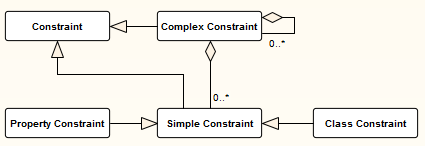
\includegraphics[width=0.60\textwidth]{images/RDF-CV-conceptual-model.png}
	\caption{\emph{RDF Constraints Vocabulary (RDF-CV)} Conceptual Model}
	\label{fig:RDF-CV-conceptual-model}
\end{figure}

We classify sets of constraints according to four dimensions.
For each constraint type, we evaluated \cite{BoschNolleAcarEckert2015} in which set of constraints their instances are contained.
%In the following, we state the rounded number of associated constraint types in brackets.
%\begin{itemize}
  %\item \emph{Universality:} \emph{specific constraints} vs. \emph{generic constraints}
	%\item \emph{Complexity:} \emph{simple constraints} vs. \emph{complex constraints}
	%\item \emph{Context:} \emph{property constraints} vs. \emph{class constraints}
	%\item \emph{DL Expressivity:} \emph{constraints expressible in DL} vs. \emph{constraints not expressible in DL}
%\end{itemize}
%(1) \emph{Universality:} \emph{specific constraints} vs. \emph{generic constraints},
%(2) \emph{Complexity:} \emph{simple constraints} vs. \emph{complex constraints},
%(3) \emph{Context:} \emph{property constraints} vs. \emph{class constraints}, and
%(4) \emph{DL Expressivity:} \emph{constraints expressible in DL} vs. \emph{constraints not expressible in DL}.

\textbf{\emph{Universality}:}
Constraints are expressible either generically (\emph{generic constraints}) using the \emph{RDF-CV}   
or specifically (\emph{specific constraints}) by domain-specific constraint languages. 
As we express constraints of each constraint type in form of \emph{generic constraints} conforming to the \emph{RDF-CV} \cite{BoschNolleAcarEckert2015},
we show that constraints of any constraint type can be described generically.

\textbf{\emph{DL Expressivity}:}
The \emph{RDF-CV} allows to describe 
constraints which are either \emph{expressible in DL} (64\%) or which are \emph{not expressible in DL} (36\%). Constraints which are expressible in DL are instantiated from 64\% of the overall 81 constraint types. On the other hand, constraints which are not expressible in DL are assigned to 36\% of all constraint types.
%In case a constraint type is \emph{expressible in DL}, we determined which DL constructs are needed to express the constraint type.

\textbf{\emph{Complexity}:}
\emph{Simple constraints} (60\% of the constraint types) denotes the set of atomic constraints. 
%which can be instantiated from almost 2/3 of the constraint types.
\emph{Complex constraints} (26\%) is the set of constraints which are created out of \emph{simple} and/or other \emph{complex constraints}.
%and which are instances of 1/4 of the constraint types.
%In case \emph{complex constraints} are expressible in DL, 
%DL statements representing \emph{complex constraints} contain DL statements standing for atomic and/or composed constraints. 
Constraints of almost 14\% of the constraint types are \emph{complex constraints} which can be simplified and therefore formulated as \emph{simple constraints} when using them in terms of syntactic sugar.

\textbf{\emph{Context}:}
\emph{Simple constraints} are applied on properties (\emph{property constraints}, 60\%),
on classes (\emph{class constraints}, 25\%), or
on properties and classes (\emph{property and class constraints}, 15\%).
%2/3 of all constraint types are types of \emph{property constraints}, 
%1/5 of \emph{class constraints}, and 
%approx. 10\% of \emph{property and class constraints}.
\emph{Simple constraints} must hold for individuals of their associated \emph{context classes}.
As \emph{context classes} of \emph{simple constraints} are reused within \emph{complex constraints},
it does not make sense to have terms standing for \emph{simple} and \emph{complex constraints} within the \emph{RDF-CV}. 
As a consequence, the distinction of \emph{property} and \emph{class constraints} is sufficient to generically describe constraints of all constraint types.
%\tb{use RDF-CV / not: expressible in RDF-CV / RDF-CV is a vocabulary, not a language}

Altogether, instances of the most of the constraint types are \emph{simple constraints on properties} which are \emph{expressible in DL}. 
%Thus, the majority of constraint types are directly and relatively easy formulated in form of \emph{simple constraints} which can be mapped to equivalent DL constructs.

\subsection{\emph{Simple Constraints}}

The implementation model of the \emph{RDF-CV} (Figure \ref{fig:RDF-CV-implementation-model}) shows that
both \emph{property constraints} and \emph{class constraints} are \emph{simple constraints}. 
%For both \emph{property} and \emph{class constraints} a \emph{context class}, a list of \emph{classes}, the \emph{constraining element}, and the \emph{constraining value} can be stated. 
%Lists of \emph{left} and \emph{right properties} can only be specified for \emph{property constraints}.
\begin{figure}[H]
	\centering
		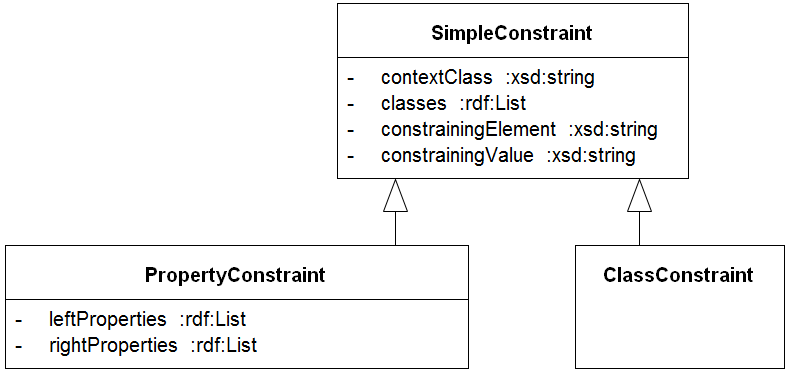
\includegraphics[width=0.80\textwidth]{images/RDF-CV-implementation-model.png}
	\caption{\emph{RDF Constraints Vocabulary (RDF-CV)} Implementation Model}
	\label{fig:RDF-CV-implementation-model}
\end{figure}
A simple constraint holds for all individuals of their associated \emph{context class}.
The \emph{minimum qualified cardinality restriction (R-75)} {\small\ms{Publication $\sqsubseteq$ $\geq$1 author.Person,}}
which restricts publications to have at least one author which must be a person,
is an example of a property constraint on \emph{author}
which holds for all individuals of the class \emph{Publication}.
Table \ref{tab:property-constraint-cardinality-restriction} displays how the property constraint is generically represented using the RDF-CV.
\begin{table}[H]
  \scriptsize
  \sffamily
  \vspace{0cm}
	\caption{Minimum Qualified Cardinality Restriction as Property Constraint}
	\label{tab:property-constraint-cardinality-restriction}
	\centering
		\begin{tabular}{c|c|c|c|c|c|c}
      \textbf{constraint set} & \textbf{context class} & \textbf{left property list} & \textbf{right p. list} & \textbf{classes} & \textbf{constraining element} & \textbf{c. value} \\
      \hline
      property & Publication & author & - & Person & $\geq$ & 1 \\
		\end{tabular}
\end{table}

%The \emph{constraining element} indicates the actual type of constraint like DL concept and role constructors ($\sqsubseteq$, $\equiv$, $\sqcap$, $\sqcup$, $\neg$, $\exists$, $\forall$, $\geq$, $\leq$), (in)equality (=, $\ne$), and further keywords for constraint types whose constraints cannot be expressed in DL (e.g., regular expressions and constraining facets). 

The \emph{constraining element} is an intuitive term which indicates the actual type of constraint. For the majority of the constraint types, there is exactly one constraining element. For the constraint type \emph{property domain (R-25, R-26)} whose constraints restrict domains of properties, e.g., there is only one constraining element with exactly the same identifier \emph{property domain}. For a few constraint types, however, one constraining element is not sufficient to describe all possible constraints of a particular constraint type and therefore multiple constraining elements may be stated. The constraint type \emph{language tag cardinality (R-48, R-49)}, for instance, is used to restrict data properties to have a minimum, maximum, or exact number of relationships to literals with selected language tags. Thus, three constraining elements are needed to express each possible constraint of that constraint type.

If constraint types are expressible in DL, associated constraining elements are formally based on DL constructs like concept and role constructors ($\sqsubseteq$, $\equiv$, $\sqcap$, $\sqcup$, $\neg$, $\exists$, $\forall$, $\geq$, $\leq$), equality (=), and inequality ($\ne$). In case constraint types cannot be expressed in DL such as \emph{data property facets (R-46)} or \emph{literal pattern matching (R-44)}, we reuse widely known terms from SPARQL (e.g., \emph{regex}) or XML Schema (e.g., \emph{minInclusive}) as constraining elements. For some constraint types like \emph{minimum qualified cardinality restrictions (R-75)}, it is more intuitive and concise to directly apply DL constructs like the \emph{at-least restriction} ($\geq$) as constraining elements. We provide a complete list of all constraining elements which can be used to express constraints of any constraint type \cite{BoschNolleAcarEckert2015}. 

In some cases, a constraint is only complete when a \emph{constraining value} is stated in addition to the constraining element
and simple constraints may refer to a list of \emph{classes}. The constraining element of the property constraint {\small\ms{Publication $\sqsubseteq$ $\geq$1 author.Person},} e.g., is \emph{$\geq$}, the constraining value is \emph{1}, and the list of classes includes the class \emph{Person} which restricts the objects of the property \emph{author} to be persons.

For property constraints, \emph{left} and \emph{right property lists} are specified.
The assignment of properties to these lists happens relative to the constraining element.
\emph{Object Property Paths} (\emph{R-55})
ensure that if an individual \emph{x} is connected by a sequence of object properties with an individual \emph{y}, 
then \emph{x} is also related to \emph{y} by a particular object property. 
As \emph{Stephen-Hawking} is the author of the book \emph{A-Brief-History-Of-Time} 
%{\small\ms{(authorOf(Stephen-Hawking, A-Brief-History-Of-Time))}} 
whose genre is \emph{Popular-Science}, 
%{\small\ms{(genre(A-Brief-History-Of-Time, Popular-Science)),}}
the object property path {\small\ms{authorOf $\circ$ genre $\sqsubseteq$ authorOfGenre}} infers that \emph{Stephen-Hawking} is an author of the genre \emph{Popular-Science}. 
%{\small\ms{(authorOfGenre(Stephen-Hawking, Popular-Science))}.}
Thus, when representing the property constraint using the RDF-CV (see Table \ref{tab:property-constraint-object-property-paths}), the properties \emph{authorOf} and \emph{genre} are placed on the left side of the constraining element \emph{property paths}
and the property \emph{authorOfGenre} on its right side. As this property constraint holds for all individuals within the data, the context class is set to the \emph{DL top concept} $\top$ which stands for the super-class of all possible classes.
\begin{table}[H]
  \scriptsize
  \sffamily
  \vspace{0cm}
	\caption{Object Property Paths as Property Constraint}
	\label{tab:property-constraint-object-property-paths}
	\centering
		\begin{tabular}{l|l|l|l|l|l|l}
      \textbf{c. set} & \textbf{context class} & \textbf{left p. list} & \textbf{right p. list} & \textbf{classes} & \textbf{c. element} & \textbf{c. value} \\
      \hline
      property & $\top$ & authorOf, genre & authorOfGenre & $\top$ & property paths & - \\
		\end{tabular}
\end{table}

There are simple constraints which are not expressible in DL but can still be described using the RDF-CV such as constraints of the type \emph{literal pattern matching} (\emph{R-44}) which restrict literals to match given patterns. The \emph{universal quantification (R-91)} {\small\ms{Book $\sqsubseteq$ $\forall$ identifier.ISBN}} ensures that books can only have valid \emph{ISBN} identifiers, i.e., strings that match a given regular expression.
%Even though, the restriction of the datatype \emph{ISBN} cannot be expressed in DL, \emph{OWL 2 DL} can be used to express the \emph{literal pattern matching} constraint:
%\begin{ex}
%ISBN a RDFS:Datatype ; owl:equivalentClass [ a RDFS:Datatype ;
    %owl:onDatatype xsd:string ; 
    %owl:withRestrictions ([ xsd:pattern "^\d{9}[\d|X]" ])] .
%\end{ex} 
%The first OWL 2 axiom explicitly declares {\em ISBN} to be a datatype. %\er{Why start from second and then first? Also better we say "owl axiom" when we talk axiom of owl, to prevent ambiguity.}\tb{resolved}
%The second OWL 2 axiom defines {\em ISBN} as an abbreviation for a datatype restriction on {\em xsd:string}. 
%The datatype {\em ISBN} can be used just like any other datatype like in the \emph{universal restriction} above.
%There are multiple use cases associated with the requirement to match literals according to given patterns (\emph{Literal Pattern Matching}\footnote{Corresponds to \emph{R-44-PATTERN-MATCHING-ON-RDF-LITERALS}}).
%The enterprise vessel, e.g.,  can only have the registry numbers "NCC-1701", "NCC-1701-A", "NCC-1701-B", "NCC-1701-C", "NCC-1701-D", or "NCC-1701-E".
%The universal restriction can be represented in DL:
%\ms{Enterprise $\sqsubseteq$ $\forall$ registryNumber.RegistryNumber}.
%The restriction of the datatype \ms{RegistryNumber}, however, cannot be expressed in DL, but OWL 2 DL can be used anyway to express the literal pattern matching constraint:
%
%\begin{ex}
%RegistryNumber
    %a rdfs:Datatype ; owl:equivalentClass [ a rdfs:Datatype ;
        %owl:onDatatype xsd:string ;
        %owl:withRestrictions ( [ xsd:pattern "NCC-1701([-][A-E])?" ] ) ] .
%\end{ex}
%The second axiom defines \ms{RegistryNumber} as an abbreviation for a datatype restriction on \ms{xsd:string}. 
%The first axiom explicitly declares \ms{RegistryNumber} to be a datatype. 
%The datatype \ms{RegistryNumber} can be used just like any other datatype like in the universal restriction above.
%The \emph{literal pattern matching} constraint validates \emph{ISBN} literals according to the regular expression causing constraint violations for triples which do not not match. 
%\ms{Janeway commandsEnterprise Voyager} and \ms{Voyager registryNumber "NCC-74656"\textasciicircum{}\textasciicircum{}RegistryNumber}, 
%but not for the triples \ms{Picard commandsEnterprise Enterprise} and \ms{Enterprise registryNumber "NCC-1701-E"\textasciicircum{}\textasciicircum{}RegistryNumber}.

Even though, constraints of the type \emph{literal pattern matching} cannot be expressed in DL, OWL 2 can be used to formulate the constraint:

\begin{ex}
ISBN a RDFS:Datatype ; owl:equivalentClass [ a RDFS:Datatype ;
    owl:onDatatype xsd:string ; 
    owl:withRestrictions ([ xsd:pattern "^\d{9}[\d|X]$" ])] .
\end{ex}\$$

The first OWL 2 axiom explicitly declares {\em ISBN} to be a datatype. %\er{Why start from second and then first? Also better we say "owl axiom" when we talk axiom of owl, to prevent ambiguity.}\tb{resolved}
The second OWL 2 axiom defines {\em ISBN} as an abbreviation for a datatype restriction on \emph{xsd:string}. 
The datatype {\em ISBN} can be used just like any other datatype like in the universal quantification above.

Table \ref{tab:simple-constraint-not-expressible-in-dl)} presents (1) in the first line how the literal pattern matching simple constraint which is not expressible in DL and (2) in the second line how the universal quantification complex constraint which is expressible in DL are represented using the RDF-CV. Thereby, the context class \emph{ISBN}, whose instances must satisfy the simple constraint, is reused within the list of classes the complex constraint refers to. The literal pattern matching constraint type introduces the constraining element \emph{regex} whose validation has to be implemented once like for any other constraining element.
%In general, validation has to be implemented once for each \emph{generic constraint type} which is not expressible in DL. 
%\begin{gcotable}
%property & Enterprise & registryNumber & - & RegistryNumber & $\forall$ & - \\
%class & RegistryNumber & - & - & xsd:string & regex & 'NCC-1701([-][A-E])?' \\
%\end{gcotable}
\begin{table}[H]
  \scriptsize
  \sffamily
  \vspace{0cm}
	\caption{Simple Constraints which are not Expressible in DL}
	\label{tab:simple-constraint-not-expressible-in-dl)}
	\centering
		\begin{tabular}{l|l|l|l|l|l|l}
      \textbf{c. set} & \textbf{context class} & \textbf{left p. list} & \textbf{right p. list} & \textbf{classes} & \textbf{c. element} & \textbf{c. value} \\
      \hline
      class & ISBN & - & - & xsd:string & regex & '\string^\text{$\backslash$d$\{9\}$[$\backslash$d$\mid$X]}\$' \\
      property & Book & identifier & - & ISBN & universal quantification & - \\
		\end{tabular}
\end{table} %\tb{Erman, can you please format the regular expression in the table above correctly?}

\subsection{\emph{Complex Constraints}}

%\emph{Complex constraints} are composed out of \emph{simple constraints} and/or \emph{complex constraints}.
Complex constraints of the constraint type \emph{context-specific exclusive or of property groups} (\emph{R-13}) restrict individuals of given classes to have all properties of exactly one of multiple mutually exclusive property groups. Publications, e.g., are either identified by an \emph{ISBN} and a title (for books) or by an \emph{ISSN} and a title (for periodical publications), but it should not be possible to assign both identifiers to a given publication. This complex constraint is expressible in \emph{ShEx}: 

\begin{ex}
Publication { 
    ( isbn string , title string ) |
    ( issn string , title string ) }
\end{ex}

As \emph{The-Great-Gatsby} is a publication with an \emph{ISBN} and a title without an \emph{ISSN}, \emph{The-Great-Gatsby} is considered as a valid publication. This complex constraint is generically expressible in DL:
%This \emph{complex constraint} is expressible specifically by \emph{ShEx} and generically by DL (and can therefore be mapped to the \emph{RDF-CV} \cite{BoschEckert2015-2}).

%Half-Klingons, e.g., either have a klingon mother and a human father or a human mother and a klingon father, which can be expressed by ShEx:

%\begin{ex}
%Half-Klingon { 
    %( klingonMother Klingon , humanFather Human ) |
    %( humanMother Human , klingonFather Klingon ) }
%\end{ex}

%\begin{ex}[commandchars=\\\{\}]
%\textit{ShEx:} Publication { ( isbn string , title string ) | ( issn string , title string ) }
%\end{ex}

%As \ms{B'Elanna Torres} is a \ms{Half-Klingon} with a klingon mother and a human father, the following data is valid:

%\begin{ex}
%BElannaTorres a Half-Klingon ;
    %klingonMother Miral ; humanFather JohnTorres .
%\end{ex}

%\begin{DL}
%rdf:type(BElannaTorres,Half-Klingon) \\
%klingonMother(BElannaTorres,Miral) \\
%klingonMother(BElannaTorres,JohnTorres)
%\end{DL}
%The \emph{complex constraint} is mapped to the \emph{RDF-CV} (see Table \ref{tab:complex-constraints}) and expressed in DL as follows:

%\begin{DL}
%Half-Klingon $\sqsubseteq$ ($\neg$E $\sqcap$ F) $\sqcup$ (E $\sqcap$ $\neg$F) \\ 
%E $\equiv$ A $\sqcap$ B \\
%F $\equiv$ C $\sqcap$ D \\
%A $\sqsubseteq$ $\geq$ 1 klingonMother.Klingon $\sqcap$ $\leq$ 1 klingonMother.Klingon \\
%B $\sqsubseteq$ $\geq$ 1 humanFather.Human $\sqcap$ $\leq$ 1 humanFather.Human \\
%C $\sqsubseteq$ $\geq$ 1 humanMother.Human $\sqcap$ $\leq$ 1 humanMother.Human \\
%D $\sqsubseteq$ $\geq$ 1 klingonFather.Klingon $\sqcap$ $\leq$ 1 klingonFather.Klingon \\
%\end{DL}

\begin{DL}
\textbf{Publication $\sqsubseteq$ ($\neg$E $\sqcap$ F) $\sqcup$ (E $\sqcap$ $\neg$F)} , E $\equiv$ A $\sqcap$ B , F $\equiv$ C $\sqcap$ D \\
A $\sqsubseteq$ $\geq$ 1 isbn.string $\sqcap$ $\leq$ 1 isbn.string , B $\sqsubseteq$ $\geq$ 1 title.string $\sqcap$ $\leq$ 1 title.string \\
C $\sqsubseteq$ $\geq$ 1 issn.string $\sqcap$ $\leq$ 1 issn.string , D $\sqsubseteq$ $\geq$ 1 title.string $\sqcap$ $\leq$ 1 title.string \\
\end{DL}

%\begin{gcotable}
%class & Half-Klingon & - & - & $\neg$E $\sqcap$ F, E $\sqcap$ $\neg$F & $\sqcup$ & - \\
%class & $\neg$E $\sqcap$ F & - & - & $\neg$E, F & $\sqcap$ & - \\
%class & E $\sqcap$ $\neg$F & - & - & E, $\neg$F & $\sqcap$ & - \\
%class & $\neg$E & - & - & E & $\neg$ & - \\
%class & E & - & - & A, B & $\sqcap$ & - \\
%class & $\neg$F & - & - & F & $\neg$ & - \\
%class & F & - & - & C, D & $\sqcap$ & - \\
%class & A & - & - & A1, A2 & $\sqcap$ & - \\
%property & A1 & klingonMother & - & Klingon & $\geq$ & 1 \\
%property & A2 & klingonMother & - & Klingon & $\leq$ & 1 \\
%class & B & - & - & B1, B2 & $\sqcap$ & - \\
%property & B1 & humanFather & - & Human & $\geq$ & 1 \\
%property & B2 & humanFather & - & Human & $\leq$ & 1 \\
%class & C & - & - & C1, C2 & $\sqcap$ & - \\
%property & C1 & humanMother & - & Human & $\geq$ & 1 \\
%property & C2 & humanMother & - & Human & $\leq$ & 1 \\
%class & D & - & - & D1, D2 & $\sqcap$ & - \\
%property & D1 & klingonFather & - & Klingon & $\geq$ & 1 \\
%property & D2 & klingonFather & - & Klingon & $\leq$ & 1 \\
%\end{gcotable}

%\begin{table}[H]
  %\scriptsize
  %\sffamily
  %\vspace{0cm}
	%\caption{Complex Constraints}
	%\label{tab:complex-constraints}
	%\centering
		%\begin{tabular}{l|l|l|l|l|l|l}
      %\textbf{c. set} & \textbf{context class} & \textbf{left p. list} & \textbf{right p. list} & \textbf{classes} & \textbf{c. element} & \textbf{c. value} \\
      %\hline
%class & Publication & - & - & $\neg$E $\sqcap$ F, E $\sqcap$ $\neg$F & $\sqcup$ & - \\
%class & $\neg$E $\sqcap$ F & - & - & $\neg$E, F & $\sqcap$ & - \\
%class & E $\sqcap$ $\neg$F & - & - & E, $\neg$F & $\sqcap$ & - \\
%class & $\neg$E & - & - & E & $\neg$ & - \\
%class & E & - & - & A, B & $\sqcap$ & - \\
%class & $\neg$F & - & - & F & $\neg$ & - \\
%class & F & - & - & C, D & $\sqcap$ & - \\
%class & A & - & - & A1, A2 & $\sqcap$ & - \\
%property & A1 & isbn & - & string & $\geq$ & 1 \\
%property & A2 & isbn & - & string & $\leq$ & 1 \\
%class & B & - & - & B1, B2 & $\sqcap$ & - \\
%property & B1 & title & - & string & $\geq$ & 1 \\
%property & B2 & title & - & string & $\leq$ & 1 \\
%class & C & - & - & C1, C2 & $\sqcap$ & - \\
%property & C1 & issn & - & string & $\geq$ & 1 \\
%property & C2 & issn & - & string & $\leq$ & 1 \\
%class & D & - & - & D1, D2 & $\sqcap$ & - \\
%property & D1 & title & - & string & $\geq$ & 1 \\
%property & D2 & title & - & string & $\leq$ & 1 \\
		%\end{tabular}
%\end{table}

%Even though, tools may generate \emph{generic constraints} automatically, this 
The DL statements demonstrate that the complex constraint is composed of many other complex constraints (\emph{minimum (R-75) and maximum qualified cardinality restrictions (R-76)}) and simple constraints (\emph{intersection (R-15/16)}, \emph{disjunction (R-17/18)}, and \emph{negation (R-19/20)}). Constraints of almost 14\% of the constraint types are complex constraints which can be simplified and therefore formulated as simple constraints when using them in terms of syntactic sugar. As \emph{exact (un)qualified cardinality restrictions (=n)} and \emph{exclusive or (XOR) of property groups} are frequently used complex constraints, we propose to simplify them in form of simple constraints. As a consequence, the \emph{context-specific exclusive or of property groups (R-13)} complex constraint is represented as a generic constraint by means of the RDF-CV more intuitively and concisely (see Table \ref{tab:simplified-complex-constraints}).

%\begin{gcotable}
%class & Half-Klingon & - & - & E, F & XOR \\
%class & E & - & - & A, B & $\sqcap$ \\
%class & F & - & - & C, D & $\sqcap$ \\
%property & A & klingonMother & - & Klingon & = & 1 \\
%property & B & humanFather & - & Human & = & 1 \\
%property & C & humanMother & - & Human & = & 1 \\
%property & D & klingonFather & - & Klingon & = & 1 \\
%\end{gcotable}

\begin{table}[H]
  \scriptsize
  \sffamily
  \vspace{0cm}
	\caption{Simplified Complex Constraints}
	\label{tab:simplified-complex-constraints}
	\centering
		\begin{tabular}{l|l|l|l|l|l|l}
      \textbf{c. set} & \textbf{context class} & \textbf{left p. list} & \textbf{right p. list} & \textbf{classes} & \textbf{c. element} & \textbf{c. value} \\
      \hline
class & Publication & - & - & E, F & XOR of property groups & - \\
class & E & - & - & A, B & intersection & - \\
class & F & - & - & C, D & intersection & - \\
property & A & isbn & - & string & = & 1 \\
property & B & title & - & string & = & 1 \\
property & C & issn & - & string & = & 1 \\
property & D & title & - & string & = & 1 \\
		\end{tabular}
\end{table}

%\emph{Complex constraints} can be simplified and therefore formulated as \emph{simple constraints} when using them in terms of syntactic sugar.
%There are three forms of \emph{OWL RBox axioms}: \emph{role inclusions}, \emph{equivalence} and \emph{disjointness}. 
%\emph{OWL} provides a variety of other axiom types: \emph{role transitivity}, \emph{symmetry}, \emph{asymmetry}, \emph{reflexivity} and \emph{irreflexivity}. 
%These axiom types are sometimes considered as basic axiom types in DL - using some suggestive notation such as
%\ms{Trans(ancestorOf)} to express that the role \emph{ancestorOf} is transitive.
%Such axioms, however, are just syntactic sugar - 
%all role characteristics can be expressed using the basic features of DL.
%
%The \emph{irreflexive object properties} constraint type (\emph{R-60}) 
%restricts that no individual is connected by a given object property to itself \cite{Kroetzsch2012}.
%With the following \emph{irreflexive object property} constraint, for instance, one can state that individuals cannot be authors of themselves:
%\begin{DL}
%\ms{$\top$ $\sqsubseteq$ $\neg$ $\exists authorOf.Self$}
%\end{DL}
%When mapped to the \emph{RDF-CV} (see Table \ref{tab:irreflexive-object-properties-as-complex-constraints}), the \emph{complex constraint} aggregates three \emph{simple constraints} (one \emph{property} and two \emph{class constraints}):
%
%%\begin{gcotable}
%%property & $\exists$ marriedTo . Self & marriedTo & - & Self & $\exists$ & - \\
%%class & $\neg$ $\exists$ marriedTo . Self & - & - & $\exists$ marriedTo . Self & $\neg$ & - \\
%%class & $\top$ & - & - & $\top$, $\neg$ $\exists$ marriedTo . Self & $\sqsubseteq$ & - \\
%%\end{gcotable}
%
%\begin{table}[H]
  %\scriptsize
  %\sffamily
  %\vspace{0cm}
	%\caption{Irreflexive Object Properties as Complex Constraints}
	%\label{tab:irreflexive-object-properties-as-complex-constraints}
	%\centering
		%\begin{tabular}{l|l|l|l|l|l|l}
      %\textbf{c. set} & \textbf{context class} & \textbf{left p. list} & \textbf{right p. list} & \textbf{classes} & \textbf{c. element} & \textbf{c. value} \\
      %\hline
%property & $\exists$ authorOf.Self & marriedTo & - & Self & $\exists$ & - \\
%class & $\neg$ $\exists$ authorOf.Self & - & - & $\exists$ authorOf.Self & $\neg$ & - \\
%class & $\top$ & - & - & $\top$, $\neg$ $\exists$ authorOf.Self & $\sqsubseteq$ & - \\
		%\end{tabular}
%\end{table}
%
%When using the \emph{OWL RBox axiom} \emph{role irreflexivity} in terms of syntactic sugar, 
%the \emph{complex constraint} can be expressed more concisely in form of a \emph{simple property constraint} with exactly the same semantics (see Table \ref{tab:irreflexive-object-properties-as-simple-constraints}):
%
%%\begin{gcotable}
%%property & $\top$ & marriedTo & - & - & irreflexive & - \\
%%\end{gcotable}
%
%\begin{table}[H]
  %\scriptsize
  %\sffamily
  %\vspace{0cm}
	%\caption{Irreflexive Object Properties as Simple Constraints}
	%\label{tab:irreflexive-object-properties-as-simple-constraints}
	%\centering
		%\begin{tabular}{l|l|l|l|l|l|l}
      %\textbf{c. set} & \textbf{context class} & \textbf{left p. list} & \textbf{right p. list} & \textbf{classes} & \textbf{c. element} & \textbf{c. value} \\
      %\hline
%property & $\top$ & authorOf & - & - & irreflexive & - \\
		%\end{tabular}
%\end{table}
The \emph{primary key properties (R-226)} constraint type is often useful to declare a given (datatype) property as the primary key of a class, so that a system can enforce uniqueness. 
Books, e.g., are uniquely identified by their \emph{ISBN}, i.e., the property \emph{isbn} is inverse functional \ms{$(\ms{funct } isbn\sp{\overline{\ }})$}
which can be represented using the RDF-CV in form of a complex constraint consisting of two simple constraints (see Table \ref{tab:primary-key-properties-as-complex-constraints}).

%\begin{gcotable}
%property & $\top$ & commandAuthorizationCode$^{-}$ & commandAuthorizationCode$^{-}$ & - & inverse & - \\
%property & $\top$ & commandAuthorizationCode$^{-}$ & - & - & functional & - \\
%\end{gcotable}

\begin{table}[H]
  \scriptsize
  \sffamily
  \vspace{0cm}
	\caption{Primary Key Properties as Complex Constraints}
	\label{tab:primary-key-properties-as-complex-constraints}
	\centering
		\begin{tabular}{l|l|l|l|l|l|l}
      \textbf{c. set} & \textbf{context class} & \textbf{left p. list} & \textbf{right p. list} & \textbf{classes} & \textbf{c. element} & \textbf{c. value} \\
      \hline
property & $\top$ & isbn$^{-}$ & isbn$^{-}$ & - & inverse property & - \\
property & Book & isbn$^{-}$ & - & - & functional property & - \\
		\end{tabular}
\end{table}

Keys, however, are even more general, i.e., a generalization of inverse functional properties \cite{Schneider2009}.
A key can be a datatype, an object property, or a chain of properties.
For these generalization purposes, as there are different sorts of keys, and as keys can lead to undecidability, 
DL is extended with a special construct \emph{keyfor} \cite{Lutz2005}.
When using keyfor (\ms{isbn keyfor Book}), 
the complex constraint can be simplified and thus formulated as a simple constraint which looks like the following in concrete RDF turtle syntax:

%\begin{gcotable}
%property & StarFleetOfficer & commandAuthorizationCode & - & - & keyfor & - \\
%\end{gcotable}

%\begin{table}[H]
  %\scriptsize
  %\sffamily
  %\vspace{0cm}
	%\caption{Primary Key Properties as Simple Constraints}
	%\label{tab:primary-key-properties-as-simple-constraints}
	%\centering
		%\begin{tabular}{l|l|l|l|l|l|l}
      %\textbf{c. set} & \textbf{context class} & \textbf{left p. list} & \textbf{right p. list} & \textbf{classes} & \textbf{c. element} & \textbf{c. value} \\
      %\hline
%property & Book & isbn & - & - & keyfor & - \\
		%\end{tabular}
%\end{table}

\begin{ex}[commandchars=\\\{\}]
[   a \textit{rdfcv:PropertyConstraint} , \textit{rdfcv:SimpleConstraint} ;
    \textit{rdfcv:contextClass} Book ; \textit{rdfcv:leftProperties} ( isbn ) ; \textit{rdfcv:constrainingElement} "keyfor" ] .
\end{ex}

Complex constraints of frequently used constraint types which correspond to DL axioms like \emph{transitivity}, \emph{symmetry}, \emph{asymmetry}, \emph{reflexivity} and \emph{irreflexivity} can also be simplified in form of simple constraints. Although, these DL axioms are expressible by basic DL features, they can also be used in terms of syntactic sugar \cite{BoschEckert2015-2}.

Constraints of the \emph{irreflexive object properties (R-60)} constraint type ensure that no individual is connected by a given object property to itself \cite{Kroetzsch2012}. With the irreflexive object property constraint {\small\ms{$\top$ $\sqsubseteq$ $\neg$ $\exists authorOf.Self$}}, e.g., one can state that individuals cannot be authors of themselves. When represented using the RDF-CV, the complex constraint aggregates three simple constraints - one property and two class constraints (see Table \ref{tab:irreflexive-object-properties-as-complex-constraints}).

%\begin{gcotable}
%property & $\exists$ marriedTo . Self & marriedTo & - & Self & $\exists$ & - \\
%class & $\neg$ $\exists$ marriedTo . Self & - & - & $\exists$ marriedTo . Self & $\neg$ & - \\
%class & $\top$ & - & - & $\top$, $\neg$ $\exists$ marriedTo . Self & $\sqsubseteq$ & - \\
%\end{gcotable}

\begin{table}[H]
  \scriptsize
  \sffamily
  \vspace{0cm}
	\caption{Irreflexive Object Properties as Complex Constraints}
	\label{tab:irreflexive-object-properties-as-complex-constraints}
	\centering
		\begin{tabular}{l|l|l|l|l|l|l}
      \textbf{c. type} & \textbf{context class} & \textbf{left p. list} & \textbf{right p. list} & \textbf{classes} & \textbf{c. element} & \textbf{c. value} \\
      \hline
property & $\exists$ authorOf.Self & authorOf & - & Self & existential quantification & - \\
class & $\neg$ $\exists$ authorOf.Self & - & - & $\exists$ authorOf.Self & negation & - \\
class & $\top$ & - & - & $\top$, $\neg$ $\exists$ authorOf.Self & sub-class & - \\
		\end{tabular}
\end{table}

When using the irreflexive object property constraint in terms of syntactic sugar, 
the complex constraint can be expressed more concisely in form of a simple property constraint with exactly the same semantics (see Table \ref{tab:irreflexive-object-properties-as-simple-constraints}):

%\begin{gcotable}
%property & $\top$ & marriedTo & - & - & irreflexive & - \\
%\end{gcotable}

\begin{table}[H]
  \scriptsize
  \sffamily
  \vspace{0cm}
	\caption{Irreflexive Object Properties as Simple Constraints}
	\label{tab:irreflexive-object-properties-as-simple-constraints}
	\centering
		\begin{tabular}{l|l|l|l|l|l|l}
      \textbf{c. type} & \textbf{context class} & \textbf{left p. list} & \textbf{right p. list} & \textbf{classes} & \textbf{c. element} & \textbf{c. value} \\
      \hline
property & $\top$ & authorOf & - & - & irreflexive property & - \\
		\end{tabular}
\end{table}

%Starfleet officers, e.g., are uniquely identified by their command authorization code (e.g. to activate and cancel auto-destruct sequences).
%It means that the property \emph{commandAuthorizationCode} is inverse functional - mapped to DL and the \emph{RDF-CV} as follows:
%
%\begin{DL}
%$(\ms{funct } commandAuthorizationCode\sp{\overline{\ }})$
%\end{DL}
%
%%\begin{gcotable}
%%property & $\top$ & commandAuthorizationCode$^{-}$ & commandAuthorizationCode$^{-}$ & - & inverse & - \\
%%property & $\top$ & commandAuthorizationCode$^{-}$ & - & - & functional & - \\
%%\end{gcotable}
%
%\begin{table}
  %\scriptsize
  %\sffamily
  %\vspace{0cm}
	%\centering
		%\begin{tabular}{l|l|l|l|l|l|l}
      %\textbf{c. type} & \textbf{context class} & \textbf{left p. list} & \textbf{right p. list} & \textbf{classes} & \textbf{c. element} & \textbf{c. value} \\
      %\hline
%property & $\top$ & commandAuthorizationCode$^{-}$ & commandAuthorizationCode$^{-}$ & - & inverse & - \\
%property & $\top$ & commandAuthorizationCode$^{-}$ & - & - & functional & - \\
		%\end{tabular}
	%\caption{Primary Key Properties as Complex Constraints}
	%\label{tab:primary-key-properties-as-complex-constraints}
%\end{table}
%
%Keys, however, are even more general, i.e., a generalization of inverse functional properties \cite{Schneider2009}.
%A key can be a datatype property, an object property, or a chain of properties.
%For this generalization purposes, as there are different sorts of key, and as keys can lead to undecidability, 
%DL is extended with \emph{key boxes} and a special \emph{keyfor} construct\cite{Lutz2005}.
%This leads to the following DL and \emph{RDF-CV} mappings (only one \emph{simple property constraint}):
%
%\begin{DL}
%commandAuthorizationCode \ms{keyfor} StarfleetOfficer
%\end{DL}

%\begin{table}
  %\scriptsize
  %\sffamily
  %\vspace{0cm}
	%\centering
		%\begin{tabular}{l|l|l|l|l|l|l}
      %\textbf{c. type} & \textbf{context class} & \textbf{left p. list} & \textbf{right p. list} & \textbf{classes} & \textbf{c. element} & \textbf{c. value} \\
      %\hline
%property & StarFleetOfficer & commandAuthorizationCode & - & - & keyfor & - \\
		%\end{tabular}
	%\caption{Primary Key Properties as Simple Constraints}
	%\label{tab:primary-key-properties-as-simple-constraints}
%\end{table}

%\begin{itemize}
  %\item domain and range
	%\item Primary Key Properties
	%\item ( Exact Qualified Cardinality Restrictions on Properties )
%\end{itemize}

%\subsection{Disjoint Classes}
%
%\begin{DL}
%Hologram $\sqcap$ Human $\sqsubseteq$ $\perp$\\
%Alternative:\\
%$Hologram \sqsubseteq \neg Human$
%\end{DL}
%
%\subsection{Minimum Qualified Cardinality Restrictions on Properties}
%
%\begin{DL}
%$FederationCaptain \sqsubseteq Federation \sqcap \geq1 commandsVessel . Vessel $
%\end{DL}

%\section{Transformations and Automatic Validation of Specific Constraints}
%\section{Transformations between Specific Constraints (Expressed by Different Constraint Languages)}
%\section{Transformations between Specific Constraints}

%\section{Validation of Specific and Generic Constraints}

\section{Related Work}

In this section, we present current languages for constraint formulation and RDF data validation\footnote{
\emph{SPARQL}: \url{http://www.w3.org/TR/sparql11-query}, 
\emph{SPIN}: \url{http://spinrdf.org},
\emph{Pellet ICV}: \url{http://clarkparsia.com/pellet/icv},
\emph{Stardog ICV}: \url{http://docs.stardog.com/#_validating_constraints},
\emph{ShEx}: \url{http://www.w3.org/Submission/shex-defn},
\emph{ReSh}: \url{http://www.w3.org/Submission/shapes},
\emph{DCMI RDF-AP}: \url{http://dublincore.org/documents/singapore-framework},
\emph{Bibframe}: \url{http://bibframe.org},
\emph{DSP}: \url{http://dublincore.org/documents/dc-dsp},
\emph{RDF Schemarama}: \url{http://swordfish.rdfweb.org/discovery/2001/01/schemarama}
%\emph{Schematron}: \url{http://www.schematron.com},
%\emph{XML Schema}: \url{http://www.w3.org/TR/xmlschema-1},
}.
\emph{SPIN}, \emph{SPARQL}, OWL 2, \emph{ShEx}, \emph{ReSh}, and \emph{DSP} are the six most promising and applied languages.
%
The query language for RDF \emph{SPARQL} is generally seen as the method of choice to validate data according to certain constraints \cite{Fuerber2010}, 
although, it is not ideal for their formulation. 
In contrast, high-level constraint languages are comparatively easy to understand and constraints can be formulated more concisely.
Declarative languages may be placed on top of \emph{SPARQL} and \emph{SPIN} when using them as implementation languages.
%
\emph{SPIN} provides a vocabulary to represent \emph{SPARQL} queries as RDF triples
and uses \emph{SPARQL} to specify logical constraints and inference rules \cite{Fuerber2010}.
%
\emph{Stardog ICV} and \emph{Pellet ICV} use OWL 2 constructs to formulate constraints.
The \emph{Pellet Integrity Constraint Validator (ICV)} is a proof-of-concept extension for the \emph{OWL 2 DL} reasoner \emph{Pellet}. 
\emph{Stardog ICV} 
validates RDF data stored in a Stardog database according to 
constraints which may be written in \emph{SPARQL}, \emph{OWL}, or \emph{SWRL}. 
%
\emph{ShEx} specifies a language whose syntax and semantics are similar to regular expressions.
\emph{ShEx} associate RDF graphs with labeled patterns called \emph{shapes} 
which are used to express formal constraints on the content of RDF graphs.
%
\emph{ReSh} defines its own vocabulary for specifying \emph{shapes} of RDF resources.
Ryman et al. define \emph{shape} as a description of the set of triples a resource is expected to contain and of the integrity constraints those triples are required to satisfy \cite{Ryman2013}. 
%
\emph{DCMI RDF Application Profiles (AP)} and \emph{Bibframe} are approaches to specify profiles for application-specific purposes. 
\emph{DCMI RDF-AP} uses \emph{DSP} as generic constraint language which is also intuitive for non-experts.
The \emph{Bibliographic Framework Initiative (Bibframe)} defines a vocabulary which has a strong overlap with \emph{DSP}.
%
Kontokostas et al. define 17 data quality integrity constraints represented as \emph{SPARQL} query templates called \emph{Data Quality Test Patterns (DQTP)} \cite{Kontokostas2014}. 
%
\emph{RDF Schemarama} 
is a proof-of-concept demonstrator based on ideas from \emph{Schematron}. 
It allows to check that RDF data has required properties and
it is based on \emph{Squish}, an SQL-ish query language for RDF, instead of \emph{SPARQL}. 
%
%\emph{Schematron} is an ISO standard for the validation and quality control of XML documents based on XPath and XSLT. 
%
%\emph{XML Schema} is the primary technology for specifying and constraining the structure of XML documents.
%
In addition to the formulation of constraints, \emph{SPIN} (open source API), \emph{Stardog ICV} (as part of the \emph{Stardog RDF database}), \emph{DQTP} (tests), \emph{Pellet ICV} (extension of \emph{Pellet OWL 2 DL} reasoner) and \emph{ShEx} offer executable validation systems using \emph{SPARQL} as implementation language.

\section{Conclusion and Future Work}

%Based on our work in the \emph{DCMI} and in cooperation with the \emph{W3C} working group, 
%we published by today 81 constraint types \cite{BoschNolleAcarEckert2015}
%which form the basis to
%lay the ground for discussions on validation
%by defining a basic terminology and classification system for RDF constraints.

Based on our work in the \emph{DCMI} and in cooperation with the \emph{W3C} working group,
we published by today 81 requirements to validate RDF data and to formulate constraints; 
each of them corresponds to a constraint type from which concrete constraints are instantiated to be checked on RDF data.
These constraint types form the basis to
lay the ground for discussions on validation
by defining a basic terminology and classification system for RDF constraints.
%
There exists no single best solution considered as high-level intuitive constraint language which enables to express constraints in an easy and concise way and which is able to meet all requirements raised by data practitioners.
Thus, the idea behind this paper is to satisfy all requirements
by representing constraints of any constraint type in a generic way using a lightweight vocabulary which consists of only a few terms.
%To show that constraints can either be represented specifically (\emph{specific constraints}) by constraint languages
%or generically (\emph{generic constraints}) by \emph{description logics (DL)},
%we mapped constraint types to DL 
%to determine which DL constructs are needed to express them \cite{BoschNolleAcarEckert2015} (Section \ref{sec:vocabulary}).

As there is no standard way to formulate constraints, 
semantically equivalent \emph{specific constraints} may be represented by a variety of languages - each of them having different syntax and semantics.
We propose transformations between semantically equivalent \emph{specific constraints}
by using the proposed vocabulary to intermediately represent constraints in a generic way
(1) to avoid the necessity to understand several languages,
(2) to resolve misunderstandings about the meaning of particular constraints, and
(3) to enhance the interoperability of constraint languages (Section \ref{sec:transformations}).

We use \emph{SPIN} as basis to develop a validation environment\footref{rdf-validator} to validate RDF data according to constraints of constraint types which are expressible by arbitrary constraint languages by mapping them to \emph{SPIN}\footref{spin-mappings} \cite{BoschEckert2014-2}.
When language designers extend constraint languages 
to be able to formulate constraints of not yet supported constraint types,
our proposal enables to reuse the validation implementation of these constraint types 
by mapping \emph{specific constraints} expressed by the language to the corresponding \emph{generic constraint}.
For any constraint language, we enable to offer a validation implementation of any constraint type out-of-the-box
by providing a \emph{SPIN} mapping
for each constraint type\footref{RDF-CV-2-SPIN}  
whose constraints are represented generically \cite{BoschEckert2015-2}. 
Furthermore, our proposal makes sure that the validation on semantically equivalent \emph{specific constraints} expressed by different languages
leads to exactly the same validation results, 
i.e., that validation is performed independently from the used language (Section \ref{sec:validation}).

It is part of future work 
(1) to extend the \emph{RDF Validator} by generating \emph{generic constraints} according to inputs of domain experts who may not be familiar with the formulation of constraints,
(2) to offer bidirectional transformations between \emph{specific constraints} expressed by the most common constraint languages and corresponding \emph{generic constraints}, and
(3) to provide translations between semantically equivalent \emph{specific constraints} expressed by the most common constraint languages by using the developed vocabulary to intermediately represent constraints.
Identifying RDF validation requirements is an ongoing process,
so the task to map constraints of new constraint types to the vocabulary.

%\begin{itemize}
	%\item to provide a GUI which generates generic constraints automatically according to inputs of domain experts who are not familiar with the formulation of constraints.
	%\item to offer bidirectional transformations between specific constraints (expressed by multiple constraint languages) and generic constraints. 
	%\item to provide translations between specific constraints (expressed by any specific constraint language) by using generic constraints as an intermediate transformation step.
%\end{itemize}

\bibliography{../../literature/literature}{}
\bibliographystyle{apacite}
\setcounter{tocdepth}{1}
%\listoftodos
\end{document}
